\documentclass[a4paper,twoside]{article}
% My LaTeX preamble file - by Nathaniel Dene Hoffman
% Credit for much of this goes to Olivier Pieters (https://olivierpieters.be/tags/latex)
% and Gilles Castel (https://castel.dev)
% There are still some things to be done:
% 1. Update math commands using mathtools package (remove ddfrac command and just override)
% 2. Maybe abbreviate \imath somehow?
% 3. Possibly format for margin notes and set new margin sizes
% First, some encoding packages and useful formatting
%--------------------------------------------------------------------------------------------
\usepackage{import}
\usepackage{pdfpages}
\usepackage{transparent}
\usepackage[l2tabu,orthodox]{nag}   % force newer (and safer) LaTeX commands
\usepackage[utf8]{inputenc}         % set character set to support some UTF-8
                                    %   (unicode). Do NOT use this with
                                    %   XeTeX/LuaTeX!
\usepackage[T1]{fontenc}
\usepackage[english]{babel}         % multi-language support
\usepackage{sectsty}                % allow redefinition of section command formatting
\usepackage{tabularx}               % more table options
\usepackage{booktabs}
\usepackage{titling}                % allow redefinition of title formatting
\usepackage{imakeidx}               % create and index of words
\usepackage{xcolor}                 % more colour options
\usepackage{enumitem}               % more list formatting options
\usepackage{tocloft}                % redefine table of contents, new list like objects
\usepackage{subfiles}               % allow for multifile documents

% Next, let's deal with the whitespaces and margins
%--------------------------------------------------------------------------------------------
\usepackage[centering,margin=1in]{geometry}
\setlength{\parindent}{0cm}
\setlength{\parskip}{2ex plus 0.5ex minus 0.2ex} % whitespace between paragraphs

% Redefine \maketitle command with nicer formatting
%--------------------------------------------------------------------------------------------
\pretitle{
  \begin{flushright}         % align text to right
    \fontsize{40}{60}        % set font size and whitespace
    \usefont{OT1}{phv}{b}{n} % change the font to bold (b), normally shaped (n)
                             %   Helvetica (phv)
    \selectfont              % force LaTeX to search for metric in its mapping
                             %   corresponding to the above font size definition
}
\posttitle{
  \par                       % end paragraph
  \end{flushright}           % end right align
  \vskip 0.5em               % add vertical spacing of 0.5em
}
\preauthor{
  \begin{flushright}
    \large                   % font size
    \lineskip 0.5em          % inter line spacing
    \usefont{OT1}{phv}{m}{n}
}
\postauthor{
  \par
  \end{flushright}
}
\predate{
  \begin{flushright}
  \large
  \lineskip 0.5em
  \usefont{OT1}{phv}{m}{n}
}
\postdate{
  \par
  \end{flushright}
}

% Mathematics Packages
\usepackage[Gray,squaren,thinqspace,cdot]{SIunits}      % elegant units
\usepackage{amsmath}                                    % extensive math options
\usepackage{amsfonts}                                   % special math fonts
\usepackage{mathtools}                                  % useful formatting commands
\usepackage{amsthm}                                     % useful commands for building theorem environments
\usepackage{amssymb}                                    % lots of special math symbols
\usepackage{mathrsfs}                                   % fancy scripts letters
\usepackage{cancel}                                     % cancel lines in math
\usepackage{esint}                                      % fancy integral symbols
\usepackage{relsize}                                    % make math things bigger or smaller
%\usepackage{bm}                                         % bold math!
\usepackage{slashed}

\newcommand\ddfrac[2]{\frac{\displaystyle #1}{\displaystyle #2}}    % elegant fraction formatting
\allowdisplaybreaks[1]                                              % allow align environments to break on pages

% Ensure numbering is section-specific
%--------------------------------------------------------------------------------------------
\numberwithin{equation}{section}
\numberwithin{figure}{section}
\numberwithin{table}{section}

% Citations, references, and annotations
%--------------------------------------------------------------------------------------------
\usepackage[small,bf,hang]{caption}        % captions
\usepackage{subcaption}                    % adds subfigure & subcaption
\usepackage{sidecap}                       % adds side captions
\usepackage{hyperref}                      % add hyperlinks to references
\usepackage[noabbrev,nameinlink]{cleveref} % better references than default \ref
\usepackage{autonum}                       % only number referenced equations
\usepackage{url}                           % urls
\usepackage{cite}                          % well formed numeric citations
% format hyperlinks
\colorlet{linkcolour}{black}
\colorlet{urlcolour}{blue}
\hypersetup{colorlinks=true,
            linkcolor=linkcolour,
            citecolor=linkcolour,
            urlcolor=urlcolour}

% Plotting and Figures
%--------------------------------------------------------------------------------------------
\usepackage{tikz}          % advanced vector graphics
\usepackage{pgfplots}      % data plotting
\usepackage{pgfplotstable} % table plotting
\usepackage{placeins}      % display floats in correct sections
\usepackage{graphicx}      % include external graphics
\usepackage{longtable}     % process long tables

% use most recent version of pgfplots
\pgfplotsset{compat=newest}

% Misc.
%--------------------------------------------------------------------------------------------
\usepackage{todonotes}  % add to do notes
\usepackage{epstopdf}   % process eps-images
\usepackage{float}      % floats
\usepackage{stmaryrd}   % some more nice symbols
\usepackage{emptypage}  % suppress page numbers on empty pages
\usepackage{multicol}   % use this for creating pages with multiple columns
\usepackage{etoolbox}   % adds tags for environment endings
\usepackage{tcolorbox}  % pretty colored boxes!


% Custom Commands
%--------------------------------------------------------------------------------------------
\newcommand\hr{\noindent\rule[0.5ex]{\linewidth}{0.5pt}}                % horizontal line
\newcommand\N{\ensuremath{\mathbb{N}}}                                  % blackboard set characters
\newcommand\R{\ensuremath{\mathbb{R}}}
\newcommand\Z{\ensuremath{\mathbb{Z}}}
\newcommand\Q{\ensuremath{\mathbb{Q}}}
%\newcommand\C{\ensuremath{\mathbb{C}}}
\renewcommand{\arraystretch}{1.2}                                       % More space between table rows (could be 1.3)
\newcommand{\Cov}{\mathrm{Cov}}
\newcommand\D{\mathrm{D}}
\newcommand*{\dbar}{\ensuremath{\text{\dj}}}

\newcommand{\incfig}[2][1]{%
    \def\svgwidth{#1\columnwidth}
    \import{./figures/}{#2.pdf_tex}
}

% Custom Environments
%--------------------------------------------------------------------------------------------
\newcommand{\lecture}[3]{\hr\\{\centering{\large\textsc{Lecture #1: #3}}\\#2\\}\hr\markboth{Lecture #1: #3}{\rightmark}}   % command to title lectures
\usepackage{mdframed}
\theoremstyle{plain}
\newmdtheoremenv[nobreak]{theorem}{Theorem}[section]
\newtheorem{corollary}{Corollary}[theorem]
\newtheorem{lemma}[theorem]{Lemma}
\theoremstyle{definition}
\newtheorem*{ex}{Example}
\newmdtheoremenv[nobreak]{definition}{Definition}[section]
\theoremstyle{remark}
\newtheorem*{remark}{Remark}
\newtheorem*{claim}{Claim}
\AtEndEnvironment{ex}{\null\hfill$\diamond$}%
% Note: A proof environment is already provided in the amsthm package
\tcbuselibrary{breakable}
\newenvironment{note}[1]{\begin{tcolorbox}[
    arc=0mm,
    colback=white,
    colframe=white!60!black,
    title=#1,
    fonttitle=\sffamily,
    breakable
]}{\end{tcolorbox}}
\newenvironment{problem}{\begin{tcolorbox}[
    arc=0mm,
    breakable,
    colback=white,
    colframe=black
]}{\end{tcolorbox}}

% Header and Footer
%--------------------------------------------------------------------------------------------
% set header and footer
\usepackage{fancyhdr}                       % header and footer
\pagestyle{fancy}                           % use package
\fancyhf{}
\fancyhead[LE,RO]{\textsl{\rightmark}}      % E for even (left pages), O for odd (right pages)
\fancyfoot[LE,RO]{\thepage}
\fancyfoot[LO,RE]{\textsl{\leftmark}}
\setlength{\headheight}{15pt}


% Physics
%--------------------------------------------------------------------------------------------
\usepackage[arrowdel]{physics}      % all the usual useful physics commands
\usepackage{feyn}                   % for drawing Feynman diagrams
%\usepackage{bohr}                   % for drawing Bohr diagrams
%\usepackage{tikz-feynman}
\usepackage{elements}               % for quickly referencing information of various elements
\usepackage{tensor}                 % for writing tensors and chemical symbols

% Finishing touches
%--------------------------------------------------------------------------------------------
\author{Nathaniel D. Hoffman}

\title{33-755 Homework 4}
\date{\today}
\begin{document}
\maketitle

\section*{1. The ``Monty Hall'' problem}
Suppose you are a guest on the game show “Let’s Make a Deal”, hosted by Monty Hall. You are given the choice of three doors: Behind one door is a car; behind the others, goats. You pick a door, say No. 1, and the host, who knows what’s behind the doors, opens another door, say No. 3, behind which is a goat. He then says to you, “Do you want to pick door No. 2?” Is it to your advantage to switch your choice? Analyze this question by defining a stochastic process on a time sequence of sample spaces. Is it a Markov process? Calculate the probability that you win a car, conditioned on choosing to switch.

\begin{tcolorbox}[breakable]
    Let us pick door number one and calculate the probabilities of each possible state.
    First, there is a $ 1/3 $ chance that we have already picked correctly. In this state, it will not matter which door is opened in the next round, switching doors will always lose.
    Secondly, there is a $ 2/3 $ chance that we have picked incorrectly, and our door houses a goat rather than a car. Once the remaining door has been opened (I say remaining because the host cannot reveal the car). In this situation, staying with our choice will always lose, while switching to the only remaining door will win.
    From this, we can find the probability, given a state corresponding to a door selection and conditioned by staying or switching, to win. If we choose to switch, our probability to win is $ 2/3 $, because there was a $ 2/3 $ chance that we initially selected the wrong door, and switching to the only other door would win. If we choose not to switch, our probability to win is $ 1/3 $, because we will only win if we chose correctly the very first time between all three doors.
    This system is Markovian. Given the initial states of being correct and being incorrect, and a time evolution which involves switching, the probability of ending in the correct state depends on your initial choice. If you started in the correct state, you will end in the incorrect state, and vice versa. There is just a higher probability to start in the incorrect state, so switching to the correct one is to your advantage.
\end{tcolorbox}

\section*{2. Beam splitter with successive measurements}
The beam splitter shown below is equipped with three detectors, $ C $, $ \Gamma $ and $ \Delta $ as shown. Initially a photon is at position 0a and the detectors are in their ready states. Photons trigger detectors as they pass (e.g. $ \ket{1c,C^0} \to \ket{2c,C^*} $).
\begin{itemize}
    \item[a] A history family $ G $ contains:
        \begin{equation}
            G_c \equiv [\psi_0] \odot [\psi_1] \odot [2c,C^*, \Gamma^0, \Delta^0] \odot [3c,C^*, \Gamma^*, \Delta^0]
        \end{equation}
        \begin{equation}
            G_d \equiv [\psi_0] \odot [\psi_1] \odot [2d,C^0, \Gamma^0, \Delta^0] \odot [3d,C^0, \Gamma^0, \Delta^*]
        \end{equation}
        where $ \ket{\psi_0} = \ket{0a,C^0, \Gamma^0, \Delta^0} $ and $ \ket{\psi_1} $ is its unitary evolution. Demonstrate that $ G_c $ and $ G_d $ are compatible and consistent.
        \begin{tcolorbox}[breakable]
            Compatibility means that $ \sum_{ \vec{\alpha}} Y^{ \vec{\alpha}} = \tilde{I} $ and consistency requires $ \bra{ \vec{\alpha}} \ket{ \vec{\beta}} = 0 \iff \vec{\alpha} \neq \vec{\beta} $. First, we can write the sum of the two histories:
            \begin{align}
                G^c \wedge G^d &= [\psi_0] + [\psi_0] - [\psi_0][\psi_0]\\
                &\odot [\psi_1] + [\psi_1] - [\psi_1][\psi_1]\\
                &\odot [2c,C^*, \Gamma^0, \Delta^0] + [2d,C^0, \Gamma^0, \Delta^0] - 0\\
                &\odot [3c,C^*, \Gamma^*, \Delta^0] + [3d,C^0, \Gamma^0, \Delta^*] - 0\\
                &= I \odot I \odot I \odot I
            \end{align} since the $ t=2 $ and $ t=3 $ states are orthogonal.

            To show consistency, we know that the chainket is proportional to the ket of the final state:
            \begin{equation}
                \ket{G^c} \propto \ket{3c,C^*, \Gamma^*, \Delta^0}
            \end{equation}
            and
            \begin{equation}
                \ket{G^d} \propto \ket{3d,C^0, \Gamma^0, \Delta^*}
            \end{equation}.
            Now we compute the inner product:
            \begin{equation}
                \bra{G^d} \ket{G^c} \propto \bra{3d,C^0, \Gamma^0, \Delta^*}\ket{3c,C^*, \Gamma^*, \Delta^0} = 0
            \end{equation}
         \end{tcolorbox}
    \item[b] Evaluate every nonvanishing chain ket and determine the probability of their corresponding histories.
        \begin{tcolorbox}[breakable]
            There are only two nonvanishing chainkets, since the particle can only go down each of the two paths and trigger the corresponding detectors:
            \begin{align}
                \ket{G^c} &= \ket{3c} \bra{3c} \underbrace{ T_{32} \ket{2c} }_{\ket{3c}} \bra{2c} \underbrace{ T_{21} \bra{1c} }_{\ket{2c}} \ket{1c} \underbrace{ T_{10} \ket{0a} }_{\frac{1}{\sqrt{2} (\ket{1c} + \ket{1d})}}\\
                &= \frac{1}{\sqrt{2}} \ket{3c, C^*, \Gamma^*, \Delta^0}
            \end{align}
            where I have employed some shorthand to write down the individual state vectors. We can then see that the probability to find the particle in this state given the initial particle on the $ a $ channel is
            \begin{align}
                &\Pr([G^c]_3\mid[0a]_0)\\&= (\bra{3c\cdots} + \bra{3d\cdots})\left(\frac{1}{2}\ket{3c\cdots} \bra{3c\cdots}\right)(\ket{3c\cdots} + \ket{3d\cdots}) = \frac{1}{2}
            \end{align}
            Similarly, $ \ket{G^d} = \frac{1}{\sqrt{2}} \ket{3d,C^0, \Gamma^0, \Delta^*} $ with probability $ \frac{1}{2} $.
        \end{tcolorbox}
    \item[c] Does the wavefunction collapse? If so, when does this happen? Contrast with the family $ F $ we discussed in class that contains
        \begin{equation}
            F_c \equiv [\psi_0] \odot [1c,C^0, \Gamma^0, \Delta^0] \odot [2c,C^*, \Gamma^0, \Delta^0] \odot [3c, C^*, \Gamma^*, \Delta^0]
        \end{equation}
        \begin{equation}
            F_d \equiv [\psi_0] \odot [1d,C^0, \Gamma^0, \Delta^0] \odot [2d,C^0, \Gamma^0, \Delta^0] \odot [3d, C^0, \Gamma^*, \Delta^*]
        \end{equation}
        \begin{tcolorbox}[breakable]
            I suppose that if we discuss this in terms of the consistent histories interpretation, there is no nonlocal wavefunction collapse. However, if we were to interpret this particle as a state described by a wavefunction, we could say that the wavefunction collapses at time $ t = 2 $, right after the first detector on the $ c $ branch. We could know what the state of this detector was by measuring the end state even if the detector was turned off. In the $ F $ family, the $ \Gamma $ detector serves only as a weak detector which tells us if the particle has gone through either path. I believe this makes the nonlocality even more evident when the wavefunction collapses at $ t = 2 $ after the $ C $ detection is made. If we were to move the $ \Delta $ detector far away, we would know its state before the particle could possibly communicate with it.
        \end{tcolorbox}
    \item[d] Use family $ G $ to evaluate, if you can, the following conditional probabilities: $ \Pr([2d]_2\mid C_2^*) $; $ \Pr([3c]_3\mid C_2^*) $; $ \Pr([ \Delta^* ]_3\mid C_2^*) $; $ \Pr([1c]_1\mid C_2^*) $. If you cannot, explain why not.
        \begin{tcolorbox}[breakable]
            \begin{equation}
                \Pr([2d]_2\mid C_2^*) = \bra{2c\cdots C^*} \ket{2d \cdots C^0} \bra{2d \cdots C^0} \ket{2c\cdots C^*} = 0
            \end{equation}
            \begin{equation}
                \Pr([3c]_3\mid C_2^*) = \bra{3c\cdots C^*}T_{32} \ket{2c\cdots C^*} \bra{2c\cdots C^*} T_{23} \ket{3c\cdots C^*} = 1
            \end{equation}
            similarly
            \begin{equation}
                \Pr([ \Delta^* ]_3\mid C_2^*) = 0
            \end{equation}
            and
            \begin{equation}
                \Pr([1c]_1\mid C_2^*) = 1
            \end{equation}
        \end{tcolorbox}
\end{itemize}
\section*{3. Destructive and nondestructive measurement}
Let $ \{\ket{s^k} \qc k = 1, \cdots, N\} $ be a complete basis set for the Hilbert space of a particle. We also have a measuring device $ M $ with its own very high dimensional Hilbert space, initially in the ready state $ M_0 $. Basis states evolve along with the measuring device according to
\begin{equation}
    (\ket{s^k} \otimes M_0) \to (\ket{s^k} \otimes M_1) \to \ket{\mathcal{N}_2^k}
\end{equation}
where $ \{\ket{\mathcal{N}^k}\} $ is a set of “pointer states” consisting of $ N $ different entangled states of the particle and measuring device. Think of each pointer state as corresponding to the needle on a meter pointing in one of $ N $ possible directions $ \hat{n}^k $ that can be observed and reported. The measurement is destructive because the state of the particle is entangled with the detector.
\begin{itemize}
    \item[a] Let the initial state of the particle be $ \ket{\psi_0} = \sum_k c_k \ket{s^k} $, with $ \sum_k \abs{c_k}^2 = 1 $, and consider histories of the type $ \{Y^{jk} = ([\psi_0] \otimes M_0) \odot ([s^j] \otimes M_1) \odot [\mathcal{N}_2^k]\} $. Demonstrate that these histories are compatible and consistent.
        \begin{tcolorbox}[breakable]
            For compatibility, we want $ \sum_{jk} Y^{jk} = \tilde{I} $, so we need $ \sum_j ([s^j] \otimes M_1) = I $. This is true because $ s^j $ is a complete basis. We also require $ \sum_k [\mathcal{N}^k] = I $. I am not sure how to perform this step.

            For completeness, we need $ \bra{Y^{jk}} \ket{Y^{lm}} = 0 \iff j \neq l \qor k \neq m$. Again, I am not sure I understand this construction, so I don't know how to show this.
        \end{tcolorbox}
    \item[b] Determine the probability to end in the $ k $th pointer state.
        \begin{tcolorbox}[breakable]
            \begin{equation}
                \Pr(\ket{\mathcal{N}^k}) = \bra{\mathcal{N}^k} \ket{\mathcal{N}^k} = \frac{1}{N}
            \end{equation}
            Honestly, this last part is a guess.
        \end{tcolorbox}
    \item[c] Determine the conditional probability the particle was in state $ j $ at time $ 1 $ given the pointer state $ k $ at time $ 2 $.
        \begin{tcolorbox}[breakable]
            \begin{align}
                \Pr([s^j M_1]_1\mid\mathcal{N}_2^k) &= \bra{\mathcal{N}_2^k} T_{21}[s^j M_1]T_{12} \ket{\mathcal{N}_2^k}\\
                &= \bra{\mathcal{N}_2^k} \ket{\mathcal{N}_2^j} \bra{\mathcal{N}_2^j} \ket{\mathcal{N}_2^k}\\
                &= \delta_{jk} \ip{\mathcal{N}_2^k}
            \end{align}
        \end{tcolorbox}
    \item[d] In a nondestructive measurement, the basis states evolve according to
        \begin{equation}
            (\ket{s^k} \otimes M_0) \to (\ket{s^k} \otimes M_1) \to (\ket{s^k} \otimes \ket{M_2^k})
        \end{equation}
        where the $ \ket{M^k} $ states are states of the measuring apparatus only. Let $ \rho_{\text{ini}} = \op{\psi_0} $ be the density operator for the initial pure state of the particle. What is the reduced density operator for the state of the particle subsequent to the measurement (irrespective of the measurement outcome)? Under what conditions is the state pure or mixed?
        \begin{tcolorbox}[breakable]
            \begin{equation}
                T \ket{\psi_0} = \ket{\psi_0} \otimes \ket{M_2^k}
            \end{equation}
            This is still a product state, so tracing over the detector state gives us the reduced density operator
            \begin{equation}
                \rho = \op{\psi_0}
            \end{equation}
            since the measurement does not change the state of the particle. This state is always pure because it is unchanged from its initial pure state.
        \end{tcolorbox}
    \item[e] Assume that the measurement outcome is $ \ket{M^k} $ for a specific $ k $. What is the reduced density operator for the particle in this case?
        \begin{tcolorbox}[breakable]
            The reduced  $ \rho $ is still $ \op{\psi_0} $ since obtaining the measurement does not effect the particle state in this case.
        \end{tcolorbox}
    \item[f] Extend the unitary time evolution from time $ 0 $ up to time $ 3 $, subsequent to the nondestructive measurement. The time evolution operator from time $ 2 $ to $ 3 $ is the identity for both the particle and the measuring apparatus. Determine the conditional probability for state $ \ket{s^j} $ at time $ 3 $ subject to the measurement $ M^k $ at time $ 2 $.
        \begin{tcolorbox}[breakable]
            \begin{align}
                \Pr([s^j]_3\mid[M^k]_2) &= \bra{s^k M^k}_2 T_{23} \ket{s^j M^j}_3 \bra{s^j M^j}_3 T_{32} \ket{s^k M^k}_2\\
                &= \abs{\ip{s^k M^k}{s^j M^j}} = \delta_{jk}
            \end{align}
        \end{tcolorbox}
\end{itemize}
\section*{4. Consistent family for weak detection. Final wording as of Thursday morning. Note minor changes to part (c).}
\begin{itemize}
    \item[a] Verify that the following figure is equivalent to the Mach-Zehnder interferometer, with the crossed arrows representing the beam splitters (e.g. $ S \ket{0a} \to (\ket{1a} + \ket{1b})/ \sqrt{2} $) etc.
        \begin{figure}[h]
            \centering
            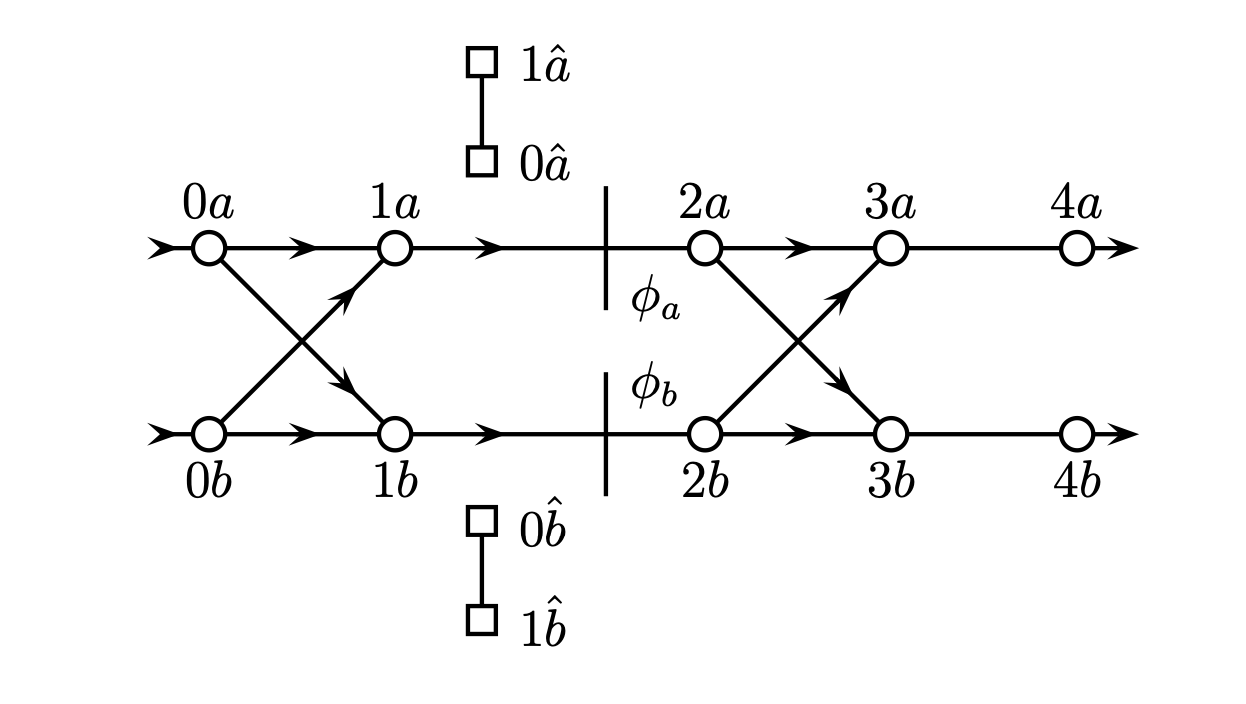
\includegraphics[width=0.7\columnwidth]{fig_hw4_4.png}
            \caption{Mach-Zehnder Interferometer}
            \label{fig:mz_inter}
        \end{figure}
        \begin{tcolorbox}[breakable]
            I'm not quite sure what is suitable for ``verification,'' but I will walk through the evolution on each channel. If we consider a particle at point $ 0a $, it is going through a beam splitter which evolves the state to a superposition of $ 1a $ and $ 1b $. The Mach-Zehnder interferometer then makes a detection on the path and adds a phase change. Somewhere in this timespan, the particle or beam hits a mirror, and at time $ 2 $, the particle hits yet another beam splitter. Both channels $ a $ and $ b $ now have an additional superposition which combines the phase changes implemented on both paths to create interference, which is read at $ t=3 $ or $ 4 $, in either exit path.
        \end{tcolorbox}
    \item[b] Verify, as claimed in class (but with $ \alpha $ and $\beta$ swapped), that $ \Pr([3a]_3) = \abs{\alpha} \sin(\Delta/2) + \abs{\beta}/2 $.
        \begin{tcolorbox}[breakable]
            \begin{align}
                \Pr([3a]_3) =& \bra{\psi_0} T_{03} [3a] T_{30} \ket{\psi_0}\\
                T_{30} \ket{\psi_0} =& T_{31} \frac{1}{\sqrt{2}} (\ket{1a} + \ket{1b})\\
                =& T_{32} ( e^{\imath \phi_a} (\alpha \ket{2a,0 \hat{a}} + \beta \ket{2a,1 \hat{a}}) \\&+ e^{\imath\phi_b} (\alpha \ket{2b,0 \hat{b}} + \beta \ket{2b,1 \hat{b}}) \\
                =& \frac{1}{2}(e^{\imath\phi_a} [\alpha (\ket{3a,0 \hat{a}} + \ket{3b,0 \hat{a}} ) + \beta (\ket{3a,1 \hat{a}} \ket{3b,1 \hat{a}})]\\
                &+ e^{\imath\phi_b} [-\alpha(\ket{3a,0 \hat{b}} + \ket{3b,0 \hat{b}})+ \beta (\ket{3a,1 \hat{b}} + \ket{3b,1 \hat{b}})])\\
                \implies & \abs{\bra{3a} T_{30} \ket{\psi_0}}^2 =\left( \frac{1}{2} e^{\imath\phi_a} (\alpha + \beta)+ e^{\imath\phi_b} (- \alpha + \beta ) \right)^2\\
                =& \abs{\alpha}^2 \sin[2]\left( \frac{\Delta}{2} \right) + \frac{\abs{\beta}^2}{2}
            \end{align}
        \end{tcolorbox}
    \item[c] Demonstrate that the following 12 histories are mutually consistent. Give an interpretation to the meaning of the set $\{Y^{(a,b;\pm;\hat{a},\hat{b})}\} $ and of the set $\{Y^{(\pm;a,b)}\}$. Note, $ \ket{\chi\pm} \equiv (\ket{1a} \pm \ket{1b}) / 2 $ and $ \ket{3\pm} \equiv (\pm \ket{3a} + \ket{3b})/2 $. As usual, some identity operators are implicit.
        \begin{tcolorbox}[breakable]
            The chainkets are proportional to their end states. Therefore,
            \begin{equation}
                \ket{Y^{(a,b;\pm)}} \propto (\pm \ket{3a} + \ket{3b}) \otimes \{\ket{1 \hat{a}}, \ket{1 \hat{b}}\}
            \end{equation}
            and
            \begin{equation}
                \ket{Y^{(\pm;a,b)}} \propto \{\ket{3a}, \ket{3b}\} \otimes \ket{0 \hat{a} 0 \hat{b}}
            \end{equation}
            The total number of chainkets seems to be reduced, but this is only because there are some in this history which vanish (such as the particle moving on path $ a $ but triggering detector $ \hat{b} $).
            \begin{equation}
                \bra{Y^{i;\pm}} \ket{Y^{(j;\pm)}} \propto (\pm \bra{3a} + \bra{3b})(\ket{3a} + \ket{3b}) \otimes \delta_{ij} \propto \delta_{ij}
            \end{equation}
            \begin{equation}
                \bra{Y^{(\pm;i)}} \ket{Y^{(\pm;j)}} \propto \bra{3i} \ket{3j} \otimes [0 \hat{a} 0 \hat{b}] = \delta_{ij} \otimes [0 \hat{a} 0 \hat{b}] \propto \delta_{ij}
            \end{equation}
            and finally
            \begin{equation}
                \bra{Y^{(i;\pm)}} \ket{Y^{(\pm;j)}} \propto \delta_{ij} \otimes \bra{1 \hat{i}}\ket{0 \hat{a} 0 \hat{b}} = \delta_{ij} \otimes 0 \propto 0
            \end{equation}
        \end{tcolorbox}

\end{itemize}

\end{document}
